\documentclass{article}

% \usepackage{lineno,hyperref}
\usepackage{graphicx}

\begin{document}

\begin{figure*}
  \centering
  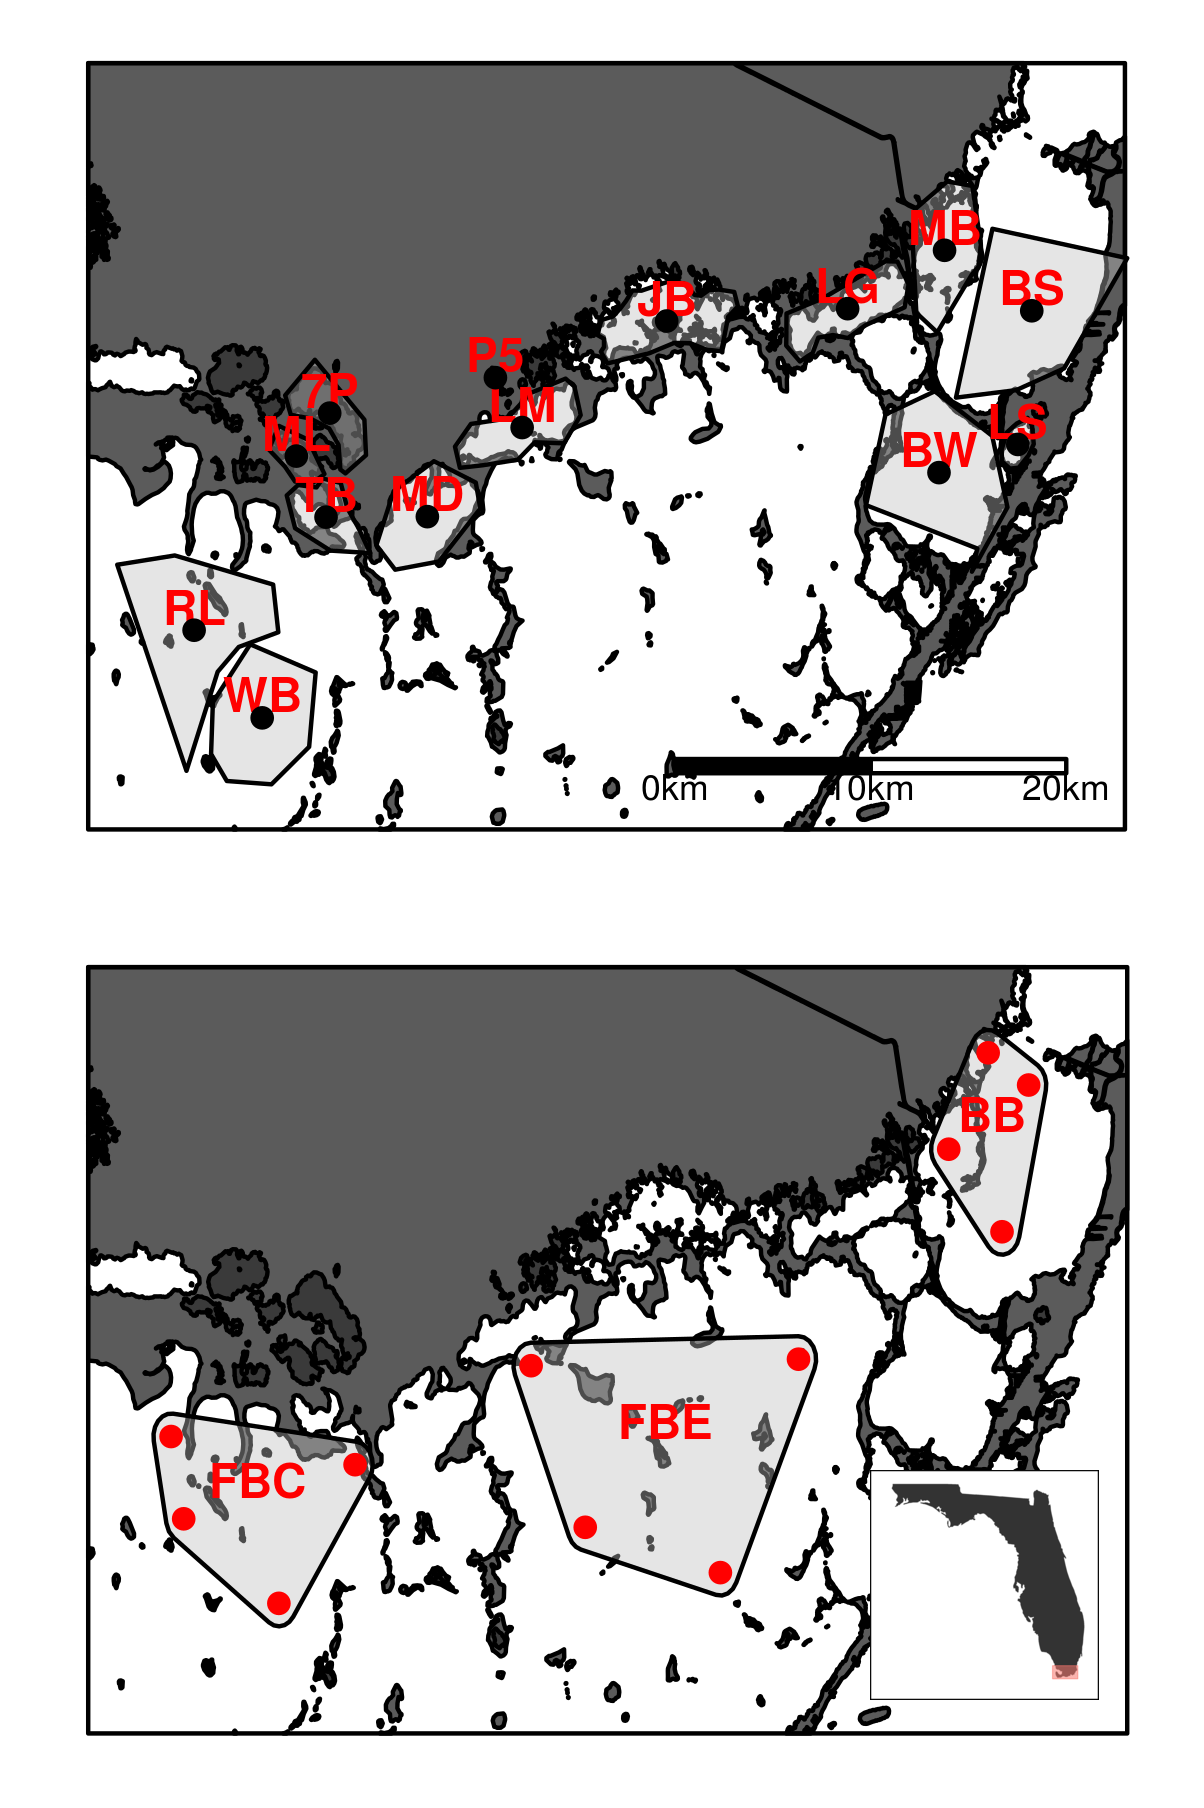
\includegraphics[width=0.75\textwidth]{../../figures/fbmap.png}
  \caption{Locations of discrete grab sampling sites within Florida Bay, USA. Polygons represent variability in sampling location over the course of the study period. a) Underway grab sampling network (1993-2015): RL = Rankin Lake, WB = Whipray Basin, TB = Terrapin Bay, ML = Monroe Lake, 7P = Seven Palm Lake, MD = Madeira Bay, LM = Little Madeira Bay, P5 = Pond Five, JB = Joe Bay, LG = Long Sound, BW = Blackwater Sound, LS = Lake Surprise, MB = Manatee Bay, BS = Barnes Sound; b) Long-term grab sampling network (2008-2015): BB – Biscayne Bay, FBE – Florida Bay East, FBC = Florida Bay Central.}
  \label{fig:1}
\end{figure*}

\newpage

\begin{figure*}
  \centering
  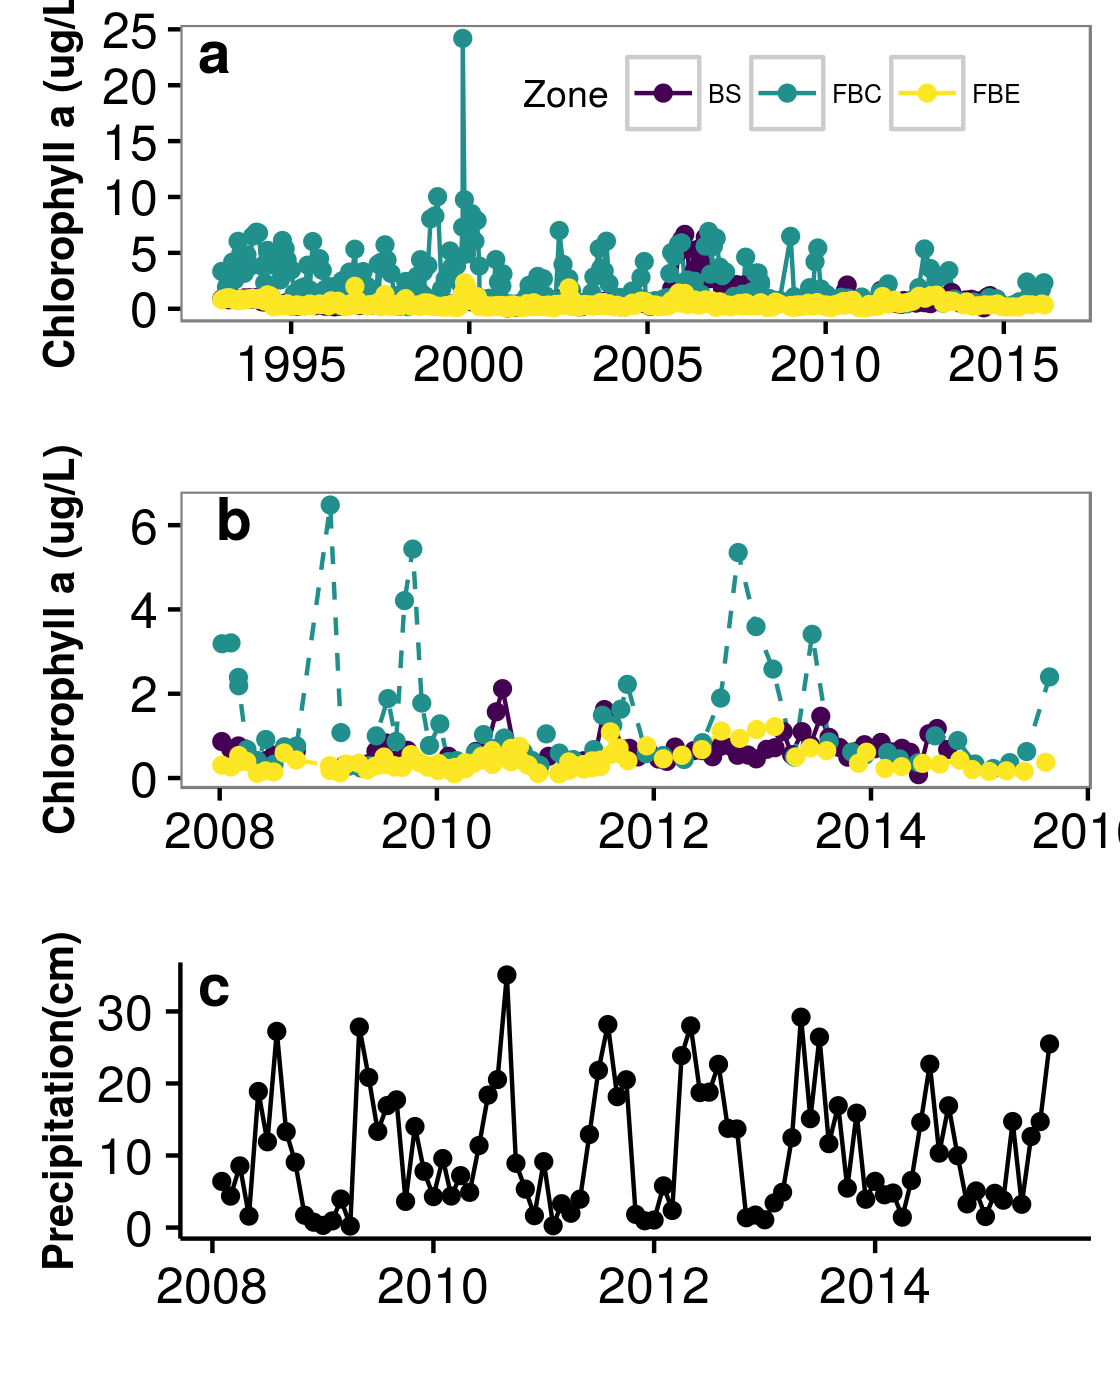
\includegraphics[width=0.75\textwidth]{../../figures/chltimeseries.png}
  \caption{a, b) Time series of average chlorophyll concentration within Florida Bay water quality zones. BS = Barnes Sound, FBC = Florida Bay Central, FBE = Florida Bay East. c) Precipitation during the study period. Precipitation data shown are cumulative monthly totals composited from three gages in the Florida Bay watershed.}
  \label{fig:2}
\end{figure*}

\newpage

\begin{figure*}
  \centering
  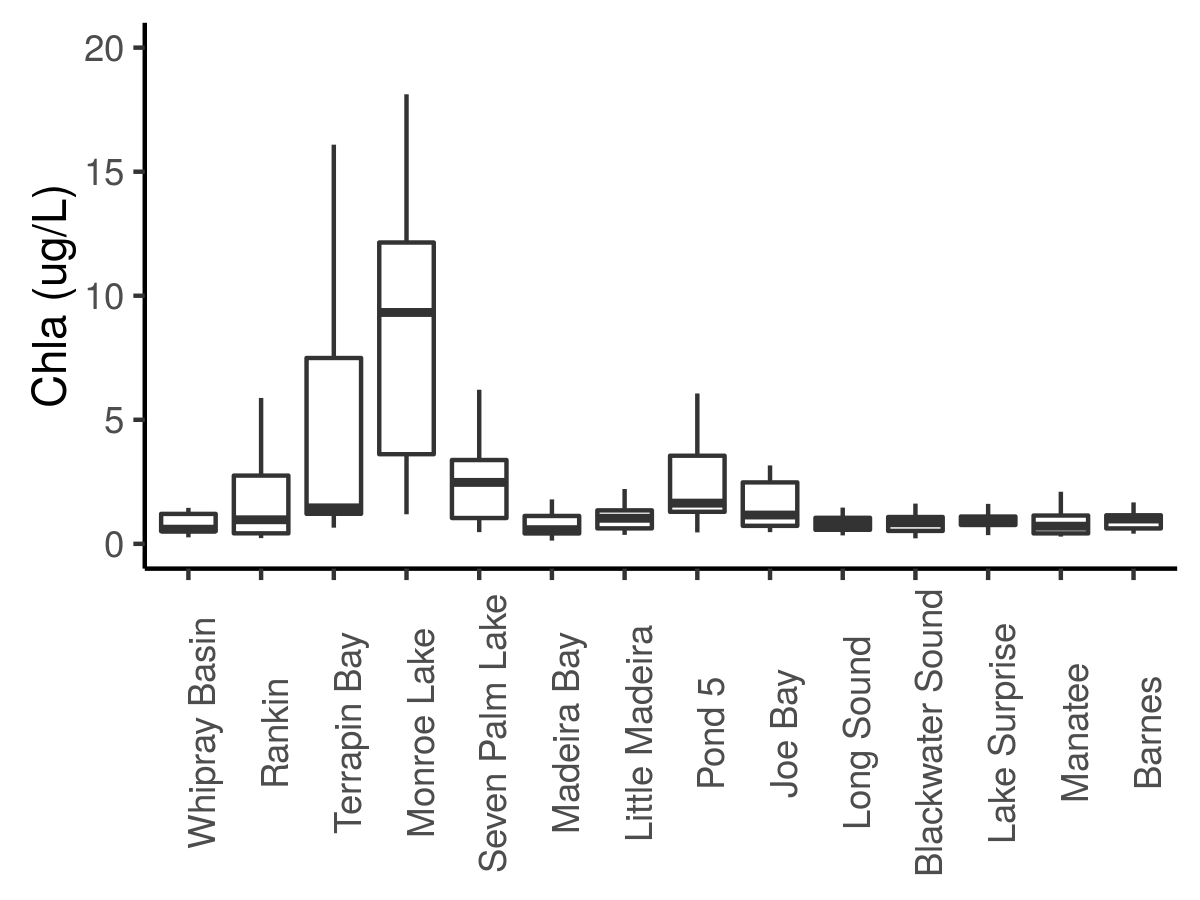
\includegraphics[width=0.75\textwidth]{../../figures/chlboxplot.png}
  \caption{Spatial distribution of chlorophyll concentration in selected Florida Bay basins. Basins are arranged geographically from west to east. The center line of each box is the median of the data, the height of the box represents the interquartile range, and the whiskers represent the fifth and 95th percentiles. }
  \label{fig:3}
\end{figure*}

\clearpage

\begin{figure*}
  \centering
  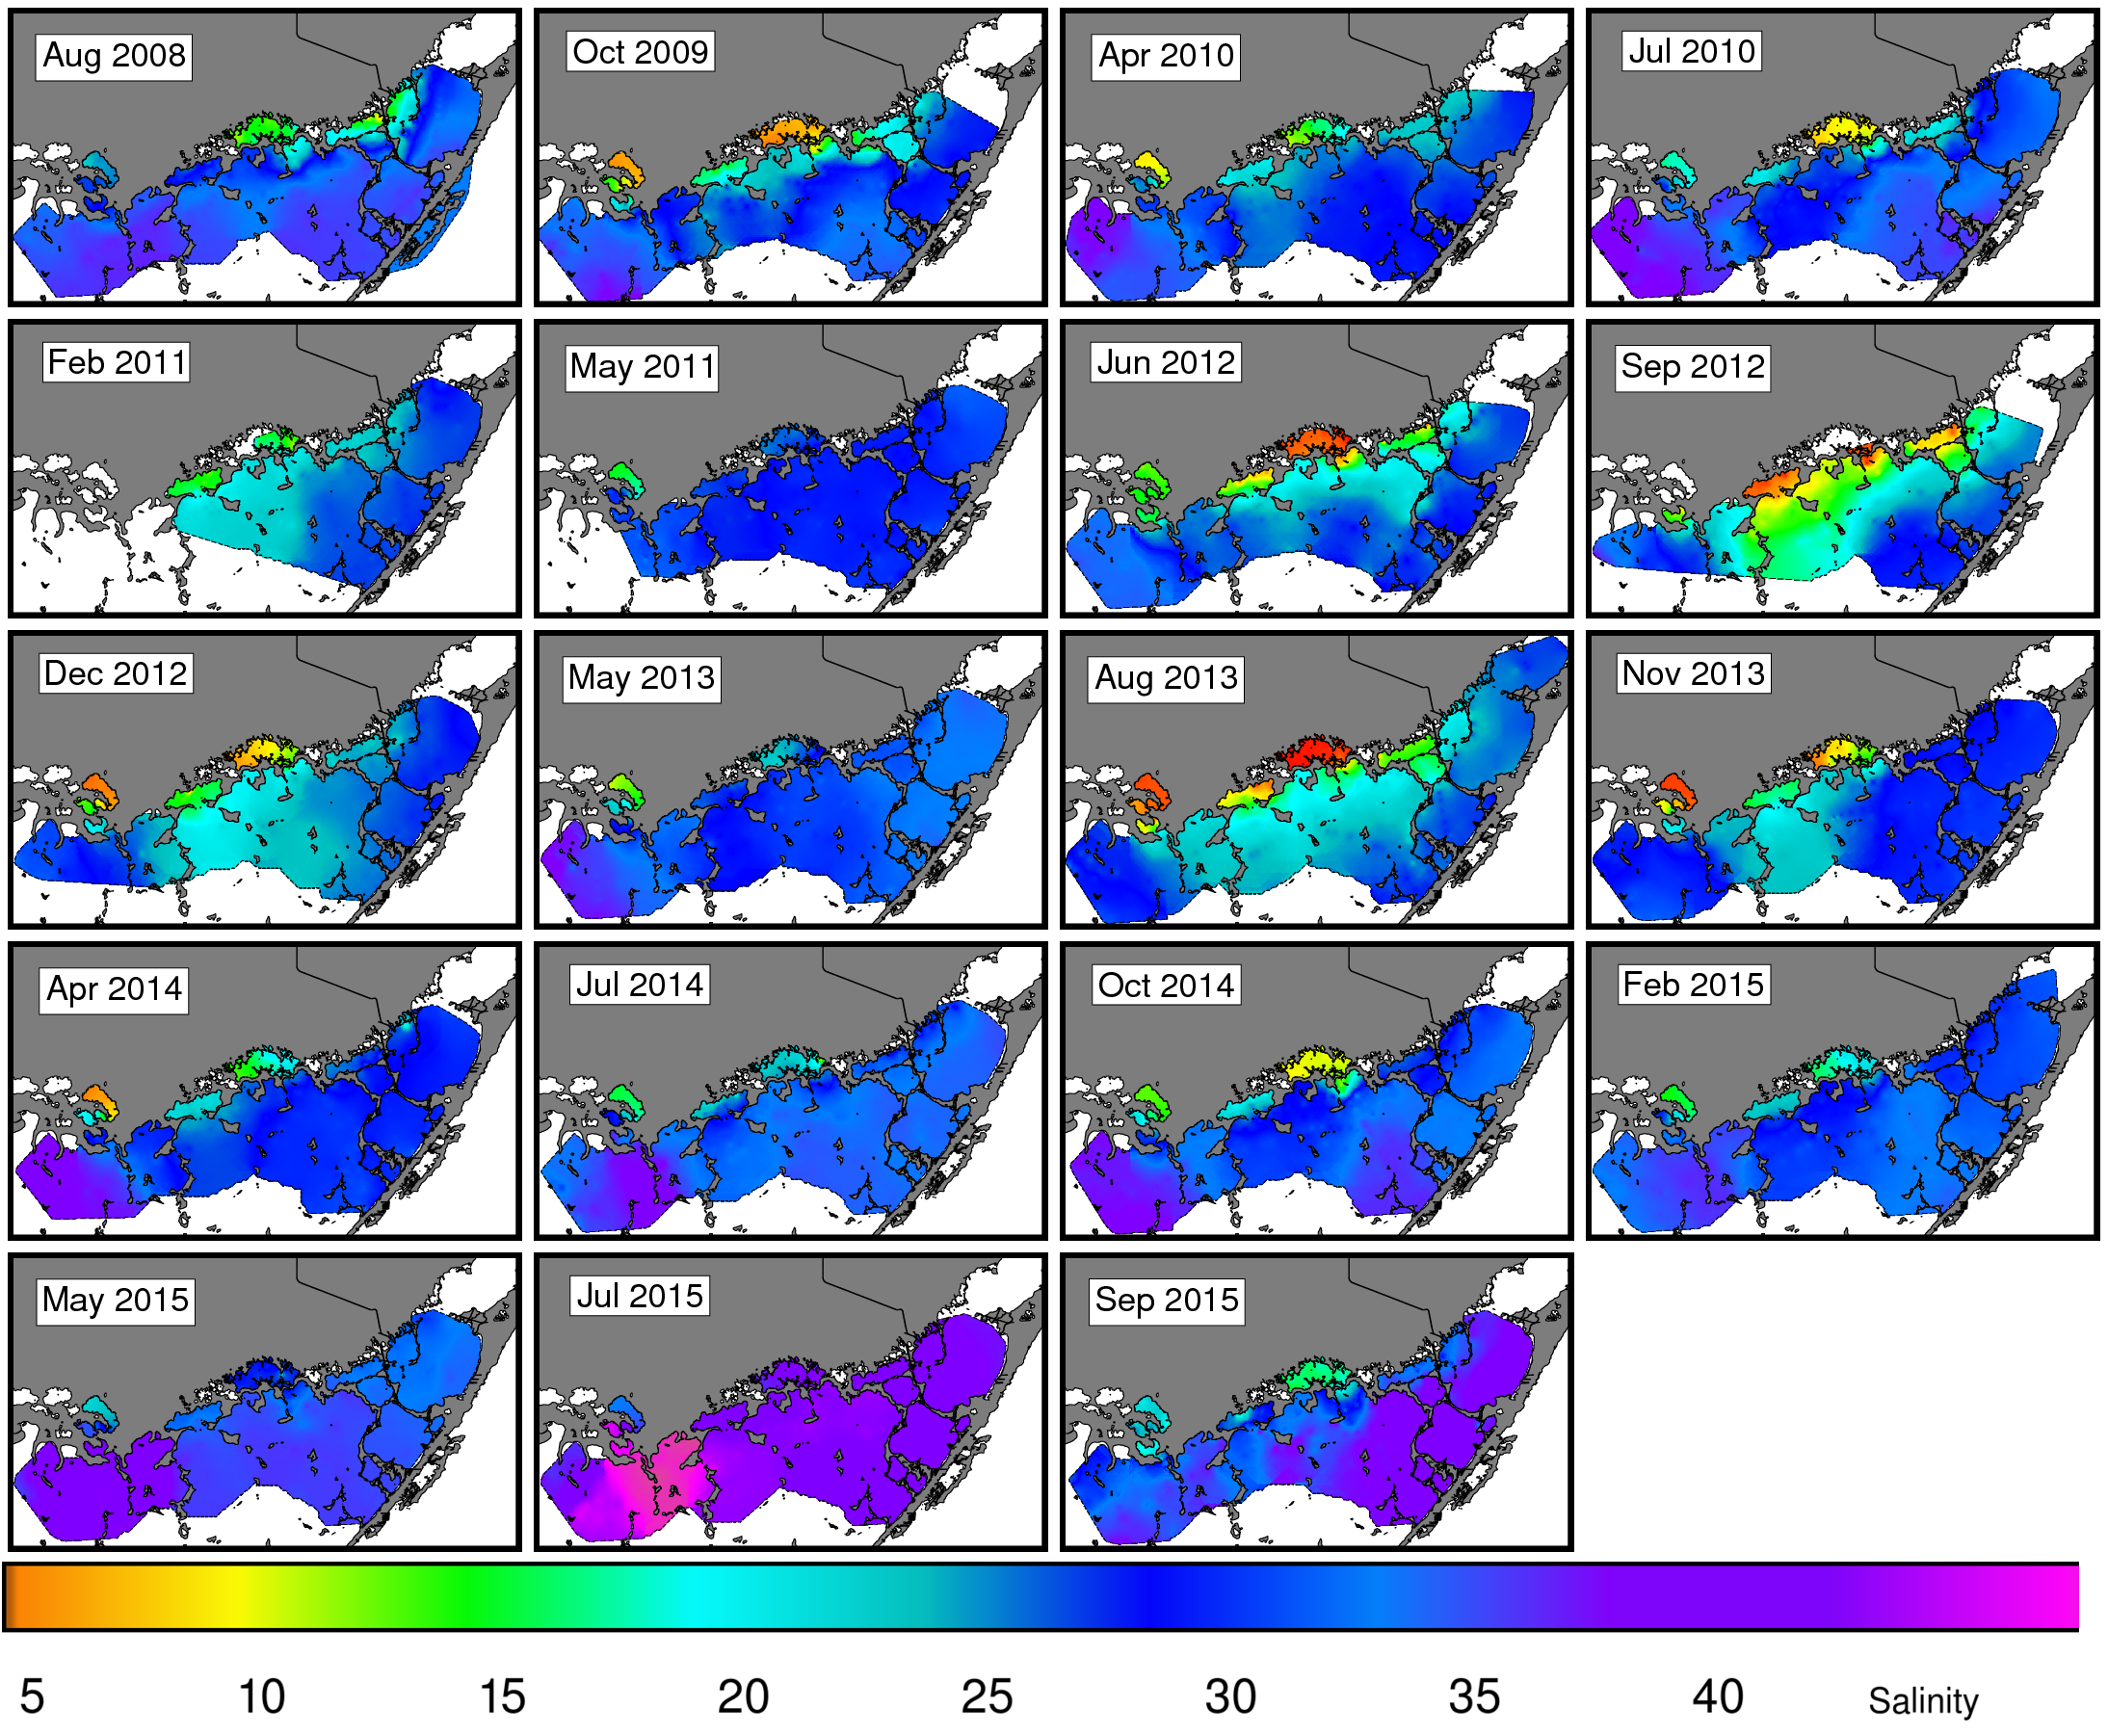
\includegraphics[width=0.9\textwidth]{../../figures/multipanel_salinity.png}
  \caption{Salinity surfaces for which a valid chlorophyll regression model could be developed. White areas denote areas that were not covered by underway surveys.}
  \label{fig:5}
\end{figure*}

\clearpage

\begin{figure*}
  \centering
  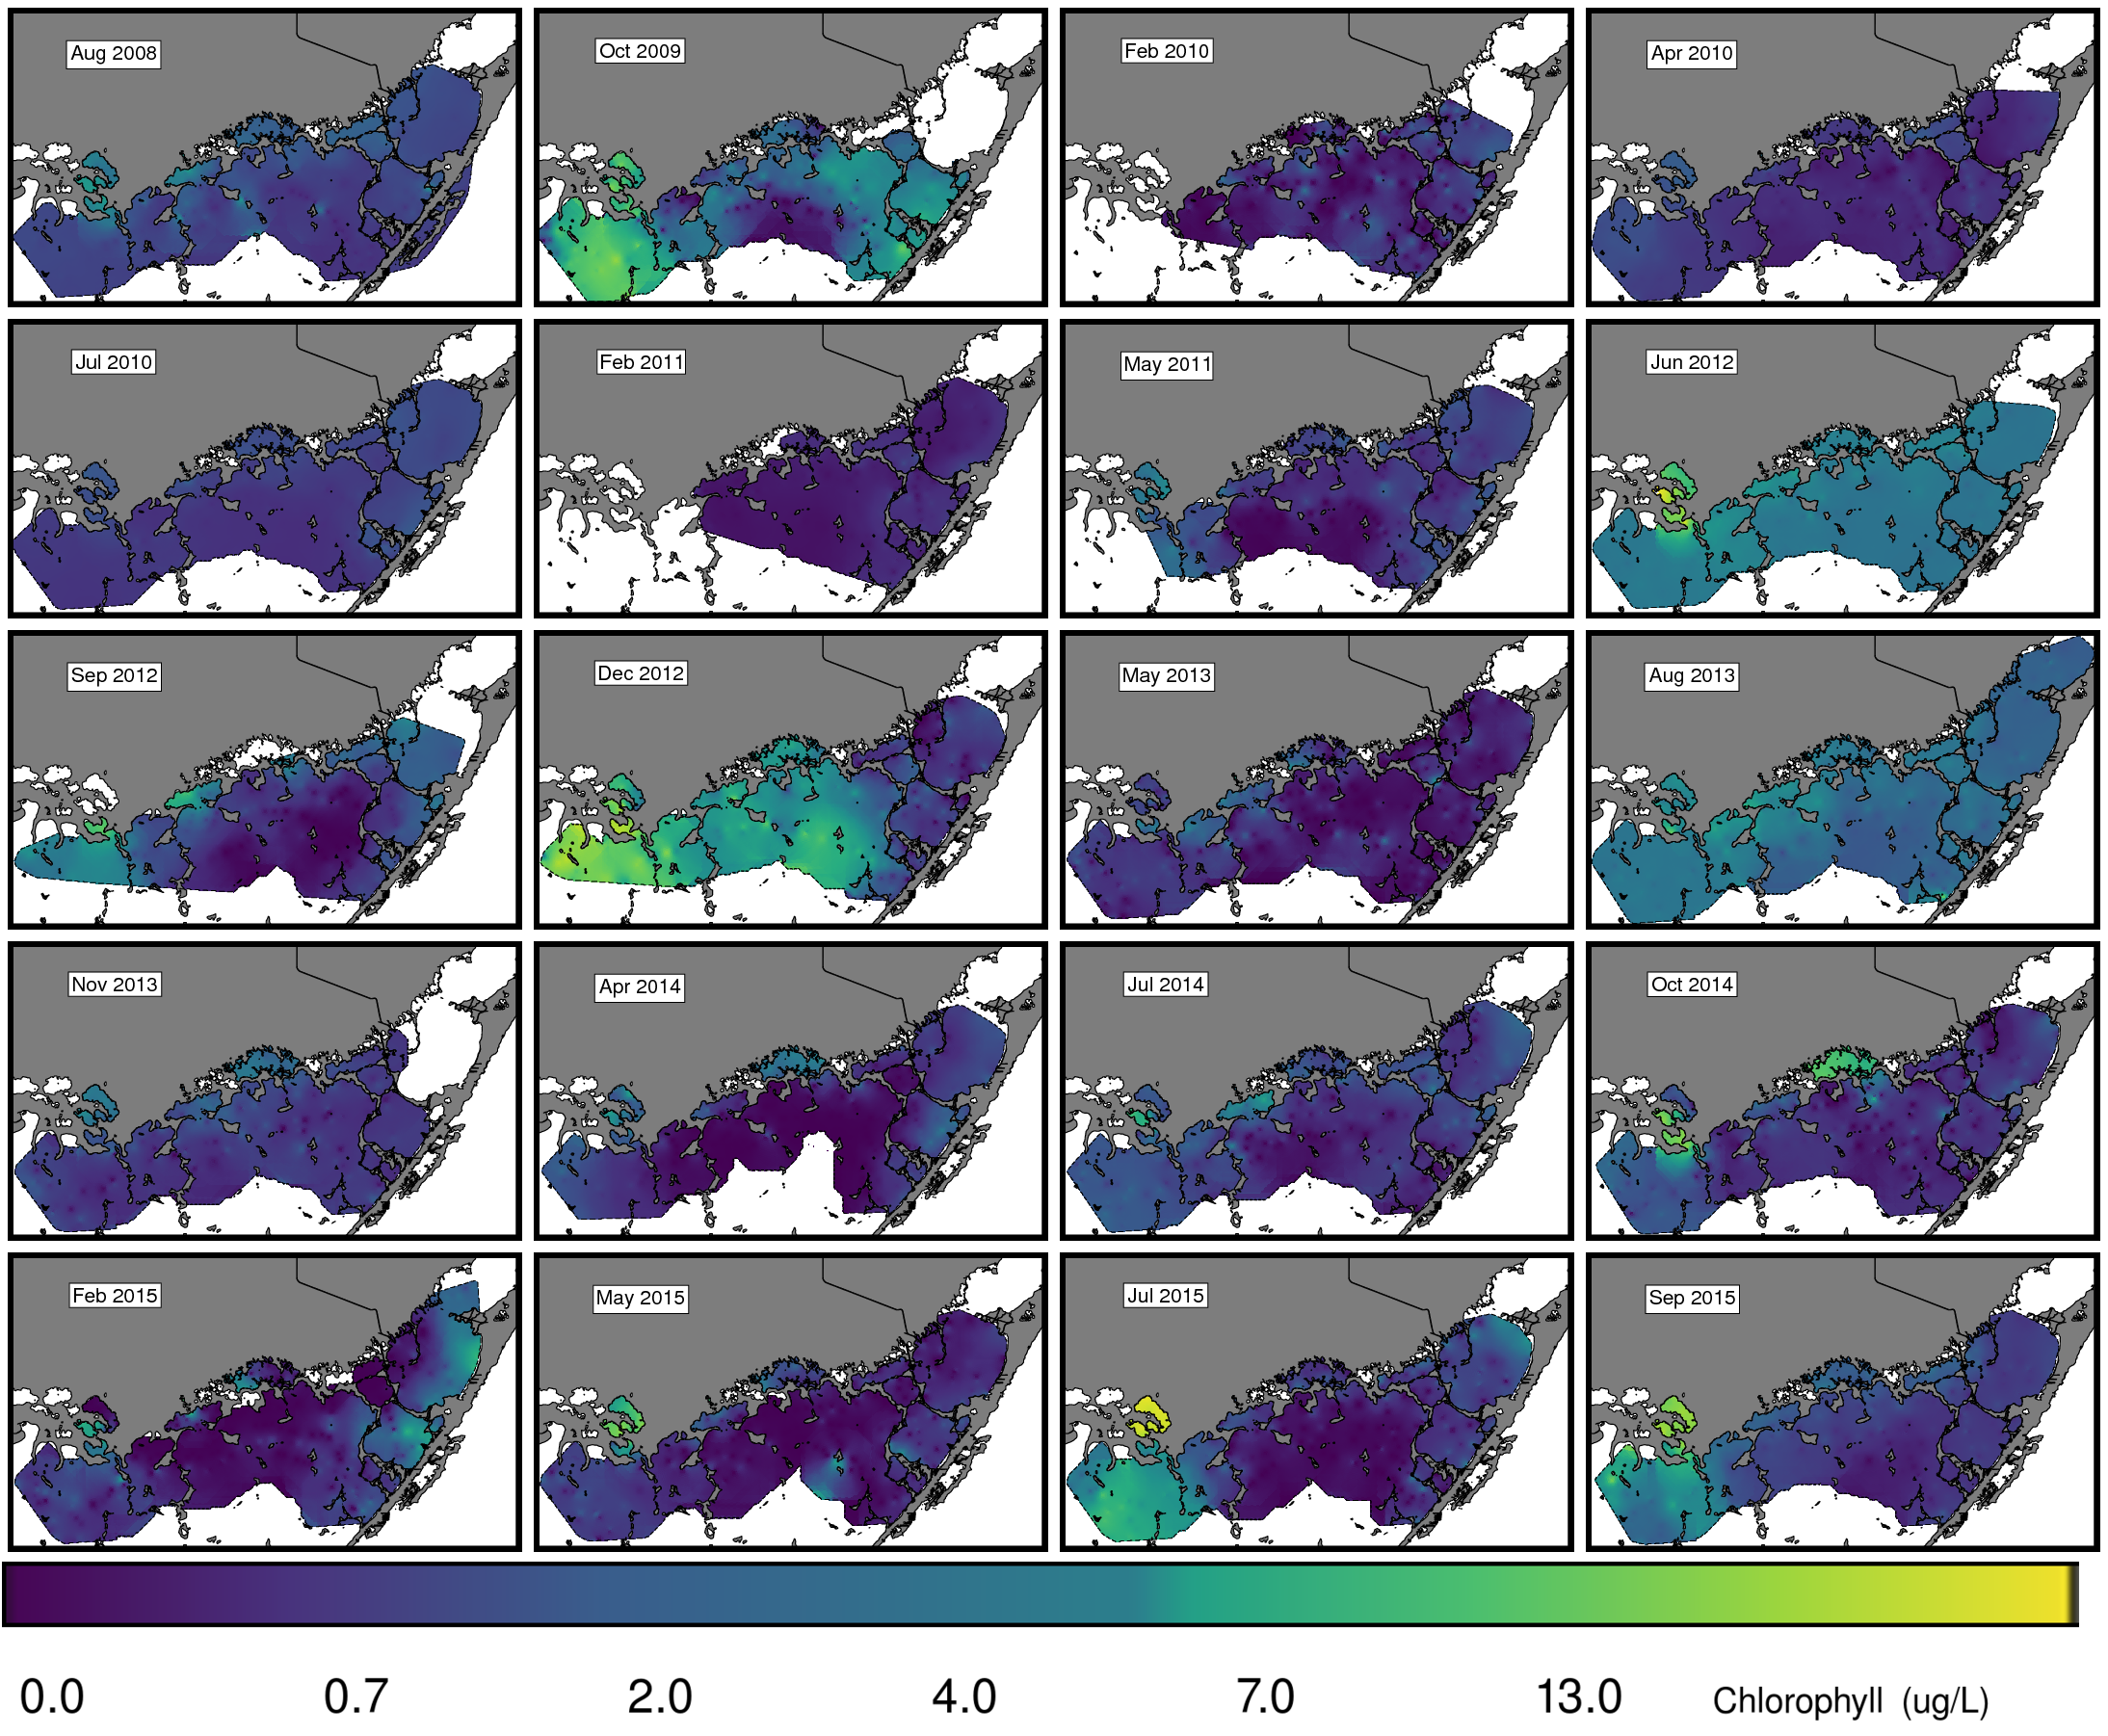
\includegraphics[width=0.9\textwidth]{../../figures/multipanel.png}
  \caption{Chlorophyll concentration surfaces calculated using the coefficients in Table 2. Surfaces shown are those for which a valid regression model could be developed. White areas denote areas that were not covered by underway surveys. Note that the color ramp is log-scaled.}
  \label{fig:4}
\end{figure*}

\clearpage

\begin{figure*}
  \centering
  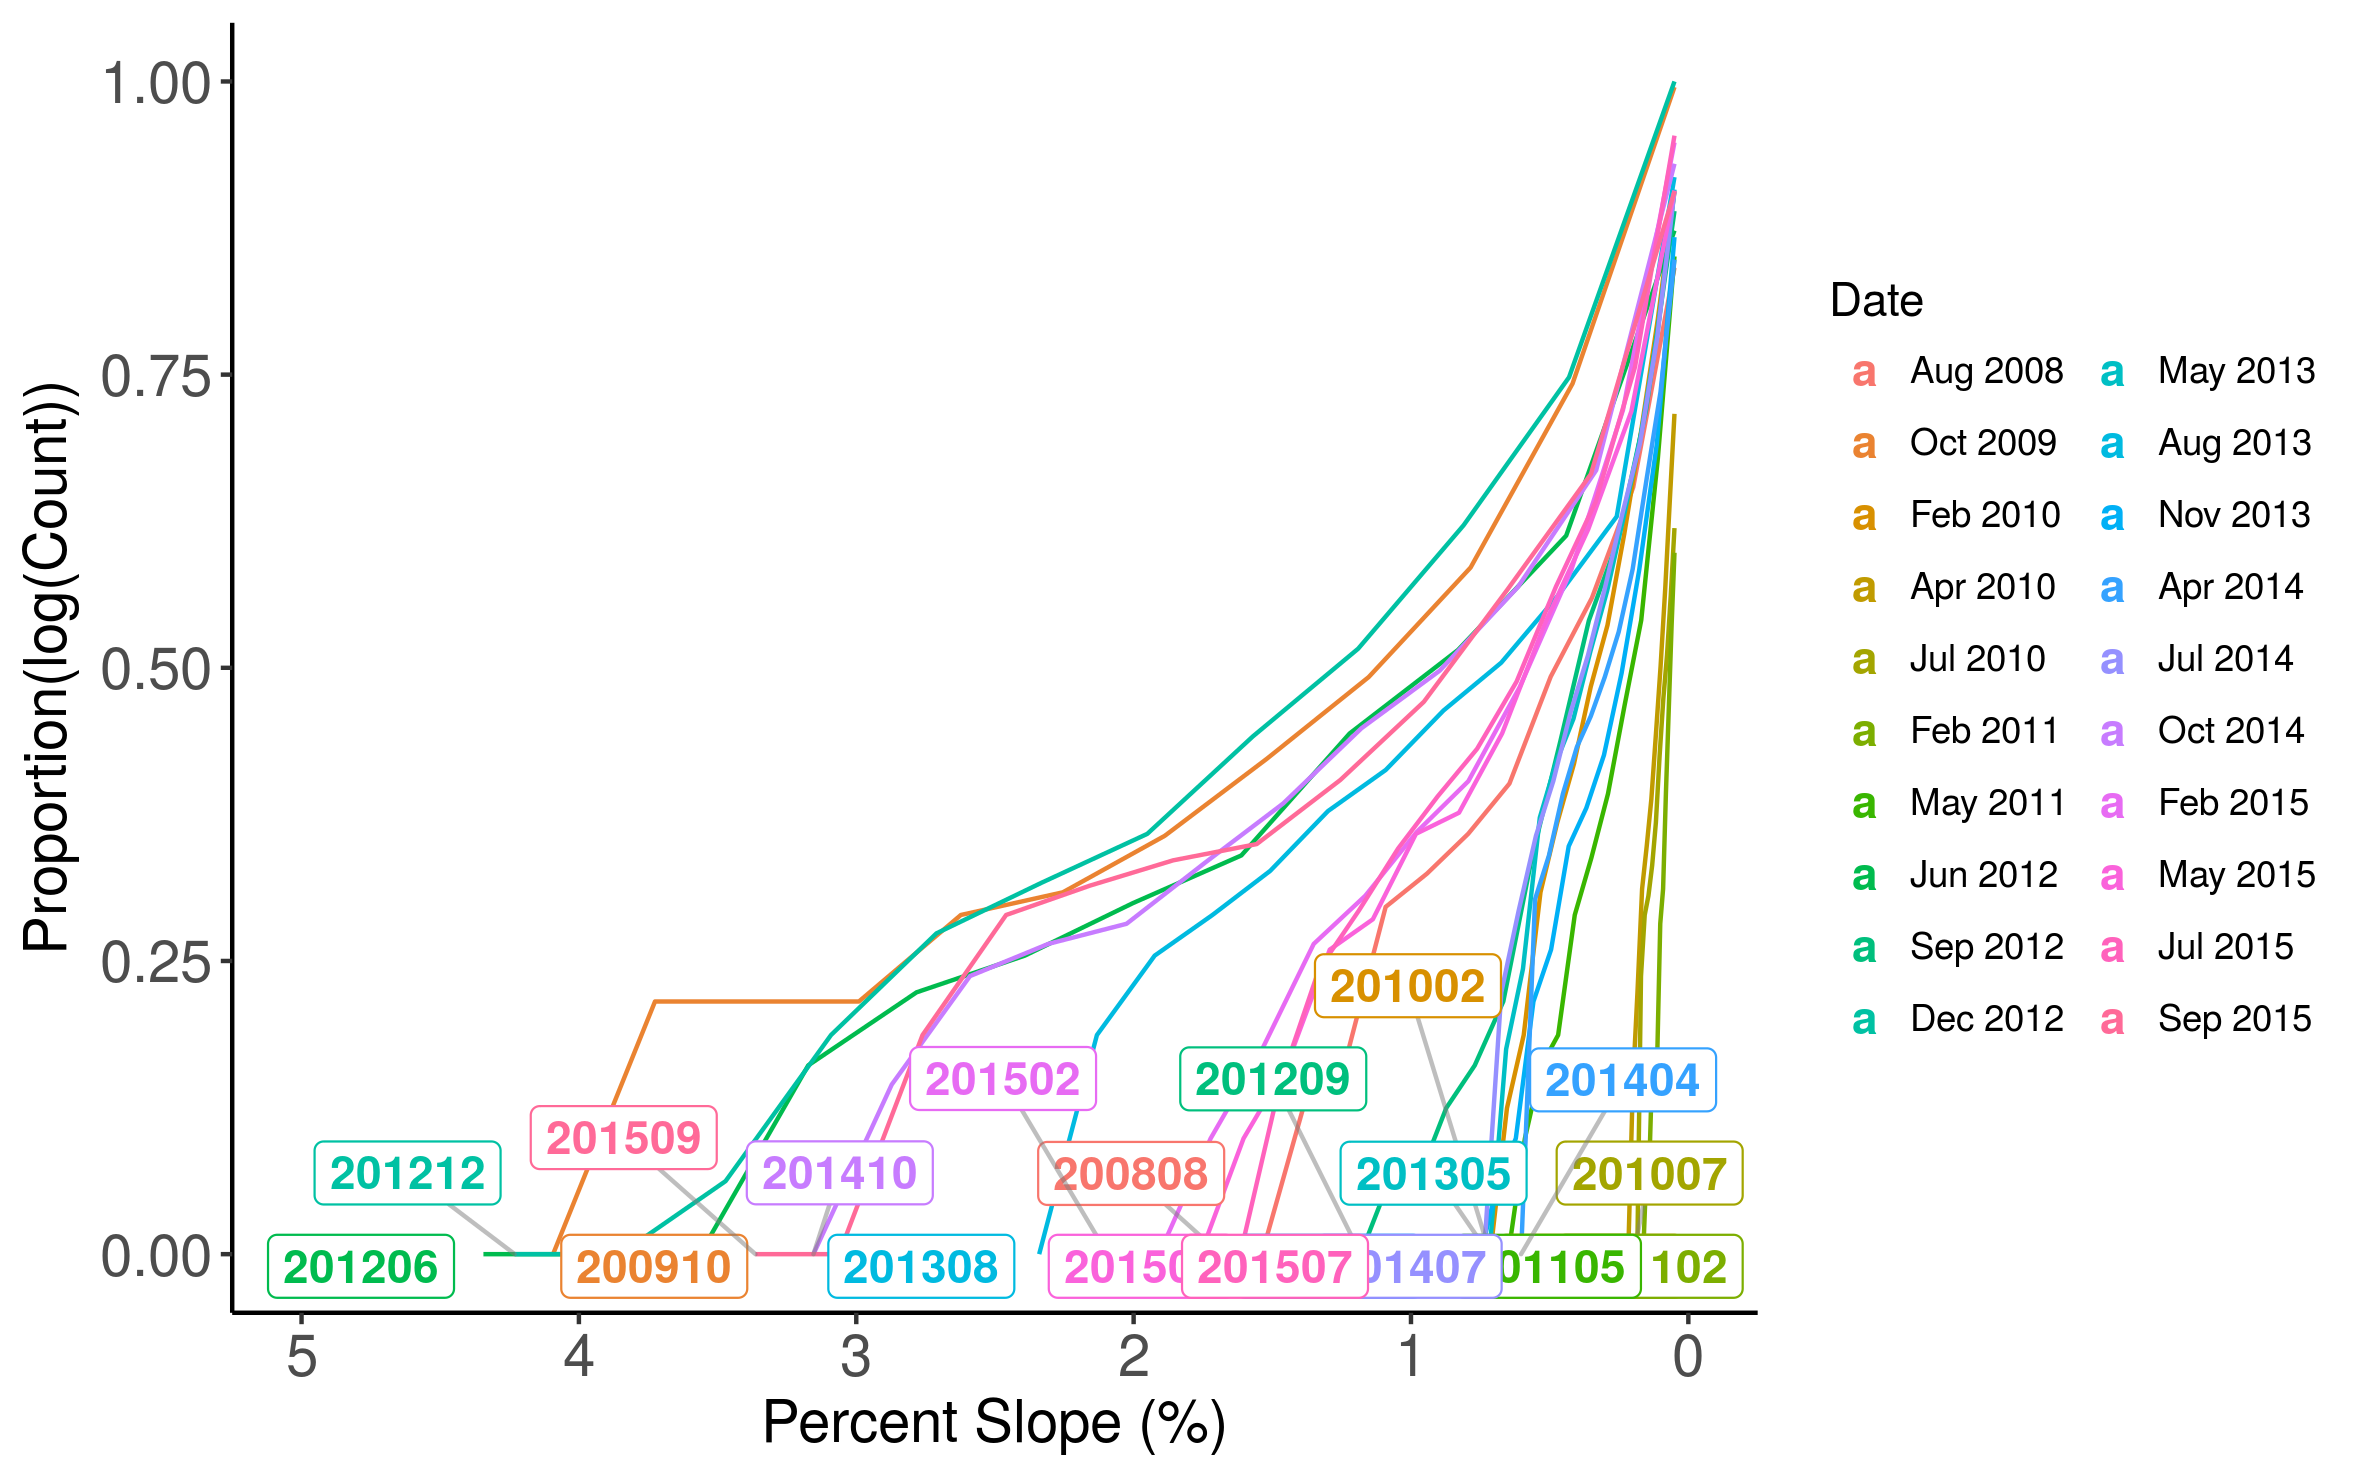
\includegraphics[width=0.85\textwidth]{../../figures/boundaries.png}
  \caption{Cumulative distribution of a) chlorophyll and b) salinity boundaries for each survey.}
  \label{fig:6}
\end{figure*}

\clearpage

% latex table generated in R 3.4.1 by xtable 1.8-2 package
% Tue Jul  4 16:26:09 2017
\begin{table}[ht]
\centering
\caption{Correlation matrix of water quality parameters for selected Florida Bay basins. TP = total phosphorus, TDP = total dissolved phosphorus, PO4 = ortho-phosphate, TN = total nitrogen, NH4 = ammonium, NO3 = nitrate, chla = chlorophyll a, PP = particulate phosphorus. $*$ indicates a significant correlation at P $<$ 0.05. Only complete cases were used in calculations (n = 86).} 
\begin{tabular}{rllllrll}
  \hline
 & TP & TDP & PO4 & TN & NH4 & NO3 & chla \\ 
  \hline
PP & 0.68* & 0.2 & 0.34* & 0.78* & 0.14 & -0.11 & 0.9* \\ 
  TP &  & 0.65* & 0.51* & 0.51* & 0.16 & 0.08 & 0.74* \\ 
  TDP &  &  & 0.48* & 0.09 & 0.18 & 0.3* & 0.28* \\ 
  PO4 &  &  &  & 0.36* & 0.16 & 0.19 & 0.4* \\ 
  TN &  &  &  &  & 0.17 & -0.12 & 0.67* \\ 
  NH4 &  &  &  &  &  & 0.55* & 0.19 \\ 
  NO3 &  &  &  &  &  &  & 0.02 \\ 
   \hline
\end{tabular}
\end{table}


\clearpage

\begin{figure*}
  \centering
  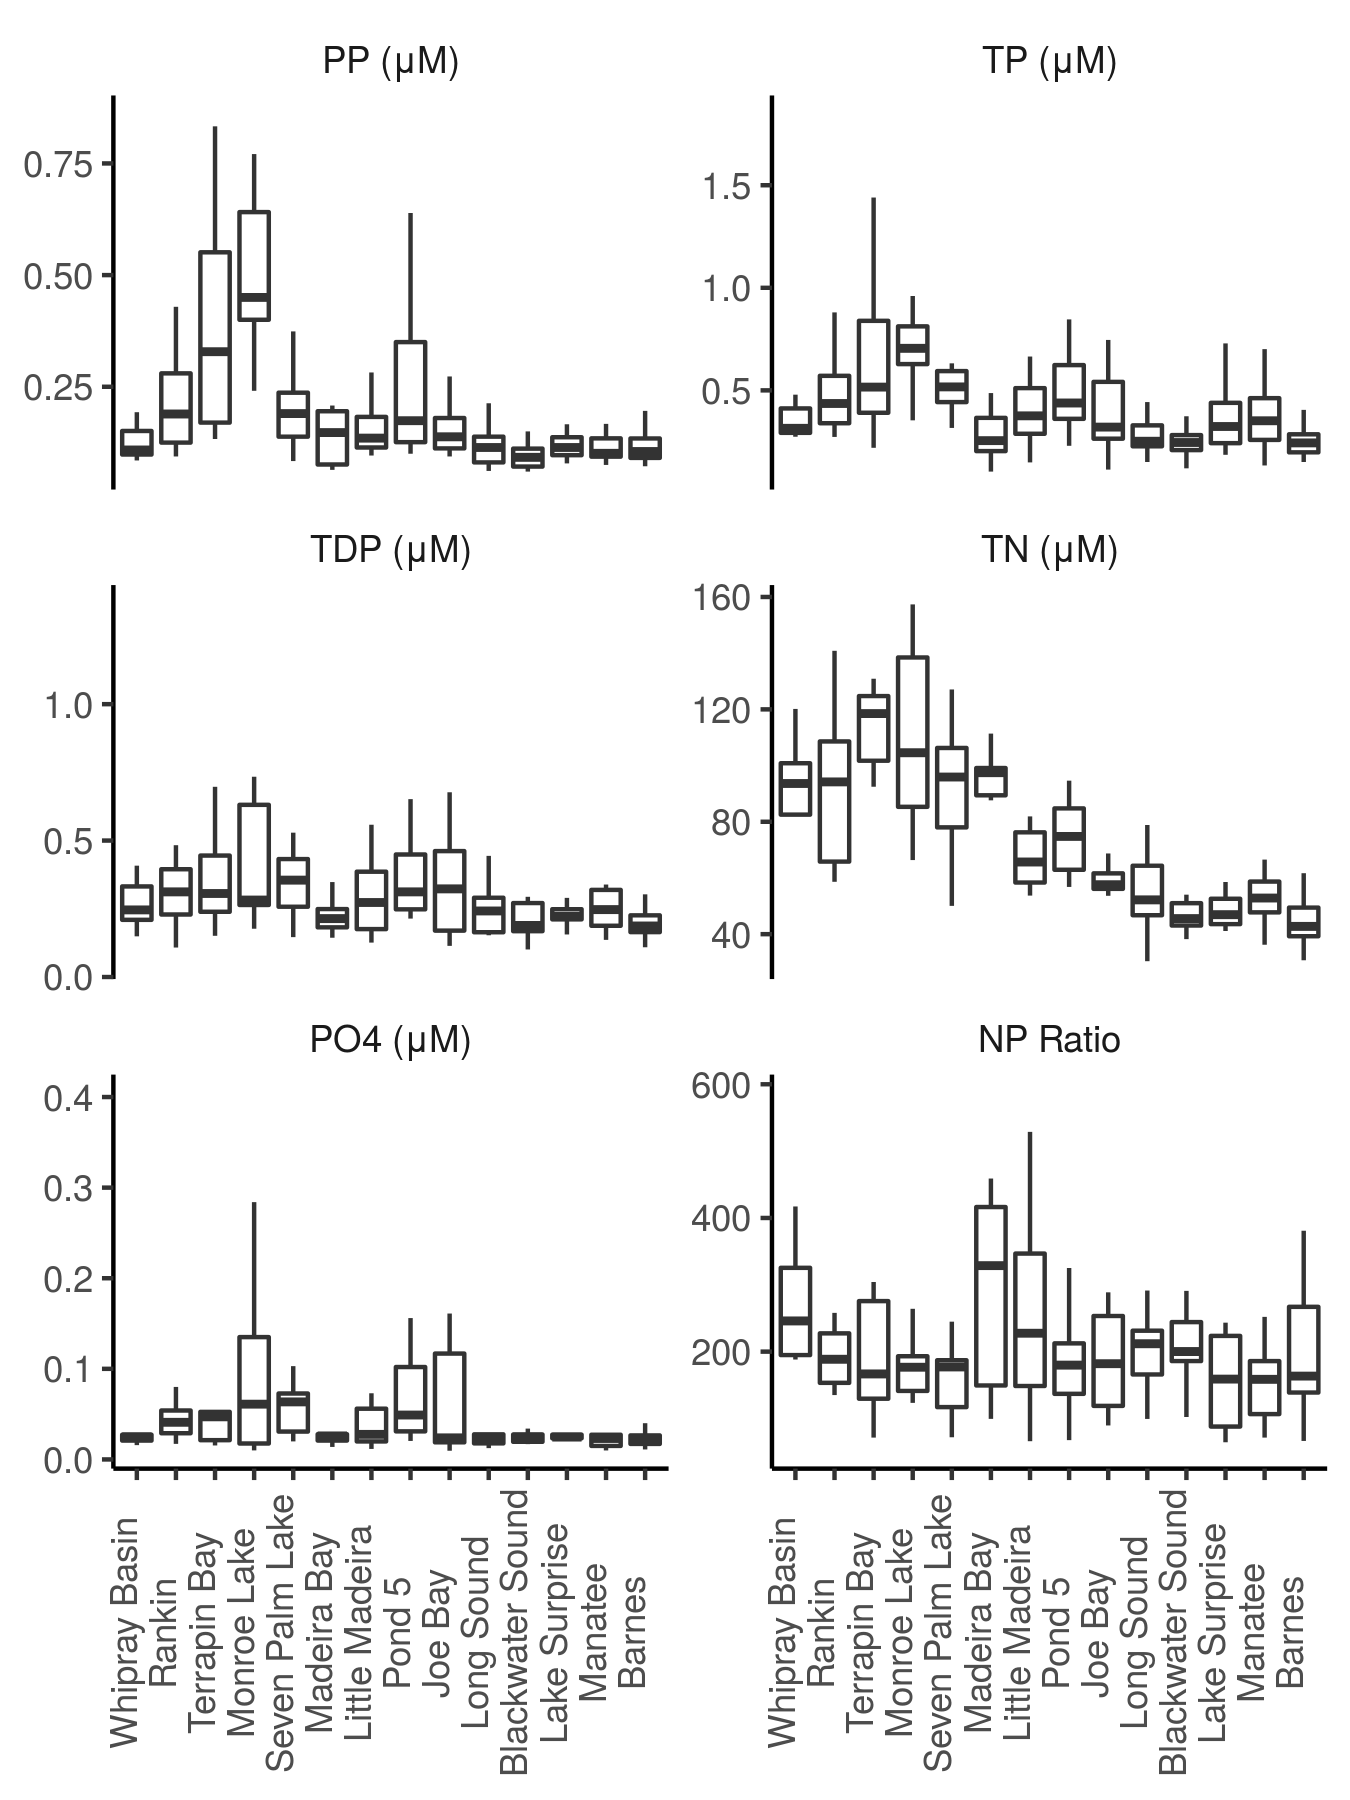
\includegraphics[width=0.75\textwidth]{../../figures/nonchlboxplot.png}
  \caption{Spatial distribution of discrete water quality parameters in selected Florida Bay basins.}
  \label{fig:7}
\end{figure*}

\newpage

\begin{table}

\caption{\label{tab:}Model coefficients for regressions between Dataflow and chlorophyll concentration of discrete grab samples. Also given is the coefficient of determination (R2) and p-value of each regression.}
\centering
\begin{tabular}[t]{lllllllllll}
\toprule
\multicolumn{1}{c}{ } & \multicolumn{2}{c}{Primary} & \multicolumn{4}{c}{Secondary} \\ \cmidrule(l{2pt}r{2pt}){2-3} \cmidrule(l{2pt}r{2pt}){4-7}
Date & CDOM & chla & PE & chla & CDOM & PC & intercept & $R^2$ & p & n\\
\midrule
2008-04 &  & 27.6258 &  &  &  &  & -4.6263 & 0.37 & 0.2 & 6\\
2008-08 &  & 5.1186 &  &  &  &  & -0.1353 & 0.9 & \textless0.01 & 10\\
2008-12 &  &  &  &  &  & 0.0509 & 0.0266 & 0.39 & 0.19 & 6\\
2009-10 & -67.1472 &  &  & 0.0495 &  &  & 6.2727 & 0.97 & \textless0.01 & 11\\
2010-02 &  &  & 0.0015 & 0.0025 & -2e-04 &  & -0.1338 & 0.63 & 0.5 & 10\\
\addlinespace
2010-04 &  & 7.8275 &  &  &  &  & -0.9164 & 0.69 & \textless0.01 & 14\\
2010-07 &  & 3.5643 &  &  &  &  & 0.0488 & 0.45 & 0.02 & 13\\
2011-02 &  &  &  & 0.0147 & -0.0011 &  & 0.0012 & 0.98 & \textless0.01 & 9\\
2011-05 &  & 12.5233 &  &  &  & 0.1473 & -3.1344 & 0.9 & \textless0.01 & 11\\
2012-06 &  &  &  &  &  & 0.0592 & 0.2531 & 0.84 & \textless0.01 & 12\\
\addlinespace
2012-09 &  & 20.2916 &  &  &  &  & -3.4262 & 0.84 & \textless0.01 & 10\\
2012-12 &  &  &  &  & 3e-04 & 0.143 & -1.2135 & 0.97 & \textless0.01 & 11\\
2013-05 &  &  &  &  &  & 0.2594 & -2.7694 & 0.96 & \textless0.01 & 14\\
2013-08 &  &  &  &  &  & 0.158 & -0.2626 & 0.68 & \textless0.01 & 15\\
2013-11 &  &  &  &  &  & 0.1864 & -1.4612 & 0.93 & \textless0.01 & 14\\
\addlinespace
2014-04 &  &  &  & 0.0217 &  &  & -1.3616 & 0.97 & \textless0.01 & 14\\
2014-07 &  &  & 0.0048 & 0.0019 &  & 0.1469 & -2.6215 & 0.91 & \textless0.01 & 14\\
2014-10 &  &  & -0.0011 &  & -5e-04 & 0.258 & -2.1036 & 0.99 & \textless0.01 & 14\\
2015-02 &  &  &  & 0.0121 & -5e-04 & 0.0485 & -0.9664 & 0.94 & \textless0.01 & 15\\
2015-05 &  &  &  &  &  & 0.2731 & -3.0247 & 0.74 & \textless0.01 & 14\\
\addlinespace
2015-07 &  &  &  &  &  & 0.3283 & -3.4682 & 0.97 & \textless0.01 & 14\\
2015-09 &  &  &  &  &  & 0.1184 & -0.8047 & 0.68 & \textless0.01 & 14\\
\bottomrule
\end{tabular}
\end{table}


\end{document}